% !TeX program = xelatex
% !TeX encoding = UTF-8
% !TeX TXS-program:compile = txs:///xelatex | txs:///xelatex
\documentclass[aspectratio=169, table, 12pt]{beamer}
% Preamble bersama seluruh slide mata kuliah ini.
% Dipanggil dari slides/sessionXX/sessionXX.tex tepat sesudah baris
% \documentclass[aspectratio=169, table, 12pt]{beamer}
% Paket tambahan yang hanya dibutuhkan satu sesi ditulis di berkas sesi itu.

\usepackage{colortbl}
\usepackage{xcolor}
\usepackage{listings}
\usepackage{tabularx}
\usepackage{booktabs}
\usepackage{tikz}
\usepackage{pgfplots}
\pgfplotsset{compat=1.18}
\usetikzlibrary{arrows.meta, positioning, calc, fit, shapes.geometric,
	shapes.multipart, backgrounds, matrix, chains, trees}

\makeatletter
\def\input@path{{../theme/}}
\makeatother
\graphicspath{{../theme/}{../../figures/}}
\usetheme{Pradita}

\definecolor{praditagreen}{RGB}{37, 113, 71}

% Tema membuat garis tabel berwarna putih. Dikembalikan agar tabel terbaca.
\arrayrulecolor{black}
\setlength{\arrayrulewidth}{0.5pt}

\lstdefinelanguage{yaml}{
	basicstyle=\ttfamily\scriptsize,
	keywordstyle=\color{blue}\bfseries,
	commentstyle=\color{gray}\itshape,
	stringstyle=\color{red},
	showstringspaces=false,
	breaklines=true,
	frame=lines,
	numbers=none,
	backgroundcolor=\color{lightgray!10},
	tabsize=2,
	morecomment=[l]{\#}
}

\lstdefinelanguage{json}{
	basicstyle=\ttfamily\scriptsize,
	stringstyle=\color{red},
	commentstyle=\color{gray},
	breaklines=true,
	showstringspaces=false,
	tabsize=2,
	numbers=none,
	frame=lines,
	backgroundcolor=\color{lightgray!10},
	string=[s]{"}{"}
}

\lstdefinelanguage{bash}{
	keywords={},
	basicstyle=\ttfamily\scriptsize,
	ndkeywords={docker, kubectl, helm, curl, git, terraform},
	ndkeywordstyle=\color{purple}\bfseries,
	sensitive=true,
	commentstyle=\color{gray},
	numbers=none,
	breaklines=true,
	frame=lines,
	backgroundcolor=\color{lightgray!10},
	tabsize=2,
	comment=[l]{\#},
	showstringspaces=false
}

\lstdefinelanguage{http}{
	keywords={GET, POST, PUT, PATCH, DELETE, HEAD, OPTIONS, HTTP},
	basicstyle=\ttfamily\scriptsize,
	keywordstyle=\color{blue}\bfseries,
	sensitive=true,
	numbers=none,
	breaklines=true,
	frame=lines,
	backgroundcolor=\color{lightgray!10},
	tabsize=2,
	showstringspaces=false
}

\subtitle{IT40613 · Digital Platform \& API Economy}
\author{\textbf{Alfa Yohannis}}


\title{\Huge Monetisasi API\\ \vspace{10pt} dan Metrik Platform}
\date{Pertemuan 12}

\begin{document}
\frame{\titlepage}

\begin{frame}
  \frametitle{Isi Pertemuan}
  \vspace{14pt}
  \begin{columns}[t]
    \column{0.5\textwidth}
    {\small\tableofcontents[sections={1-6}]}

    \column{0.5\textwidth}
    {\small\tableofcontents[sections={7-11}]}
  \end{columns}
\end{frame}

\begin{frame}{\hfill}
  \centering
  \Huge{\textbf{Panggilan API naik 50 persen.\\Janji temu selesai turun.\\Apakah platform tumbuh?}}
\end{frame}

\section{Tujuan dan Konteks}

\begin{frame}{{\Large Tujuan Pembelajaran}}
  \vspace{10pt}
  \begin{itemize}
    \item Membedakan nilai API langsung dan tidak langsung beserta contoh penerapannya.
    \item Memilih model harga API yang sesuai dengan strategi platform dan sisi pasar.
    \item Menyusun pohon metrik yang menghubungkan aktivitas API dengan tujuan bisnis.
  \end{itemize}
\end{frame}

\begin{frame}{{\Large Diagram Konsep Bab 12}}
  \centering
  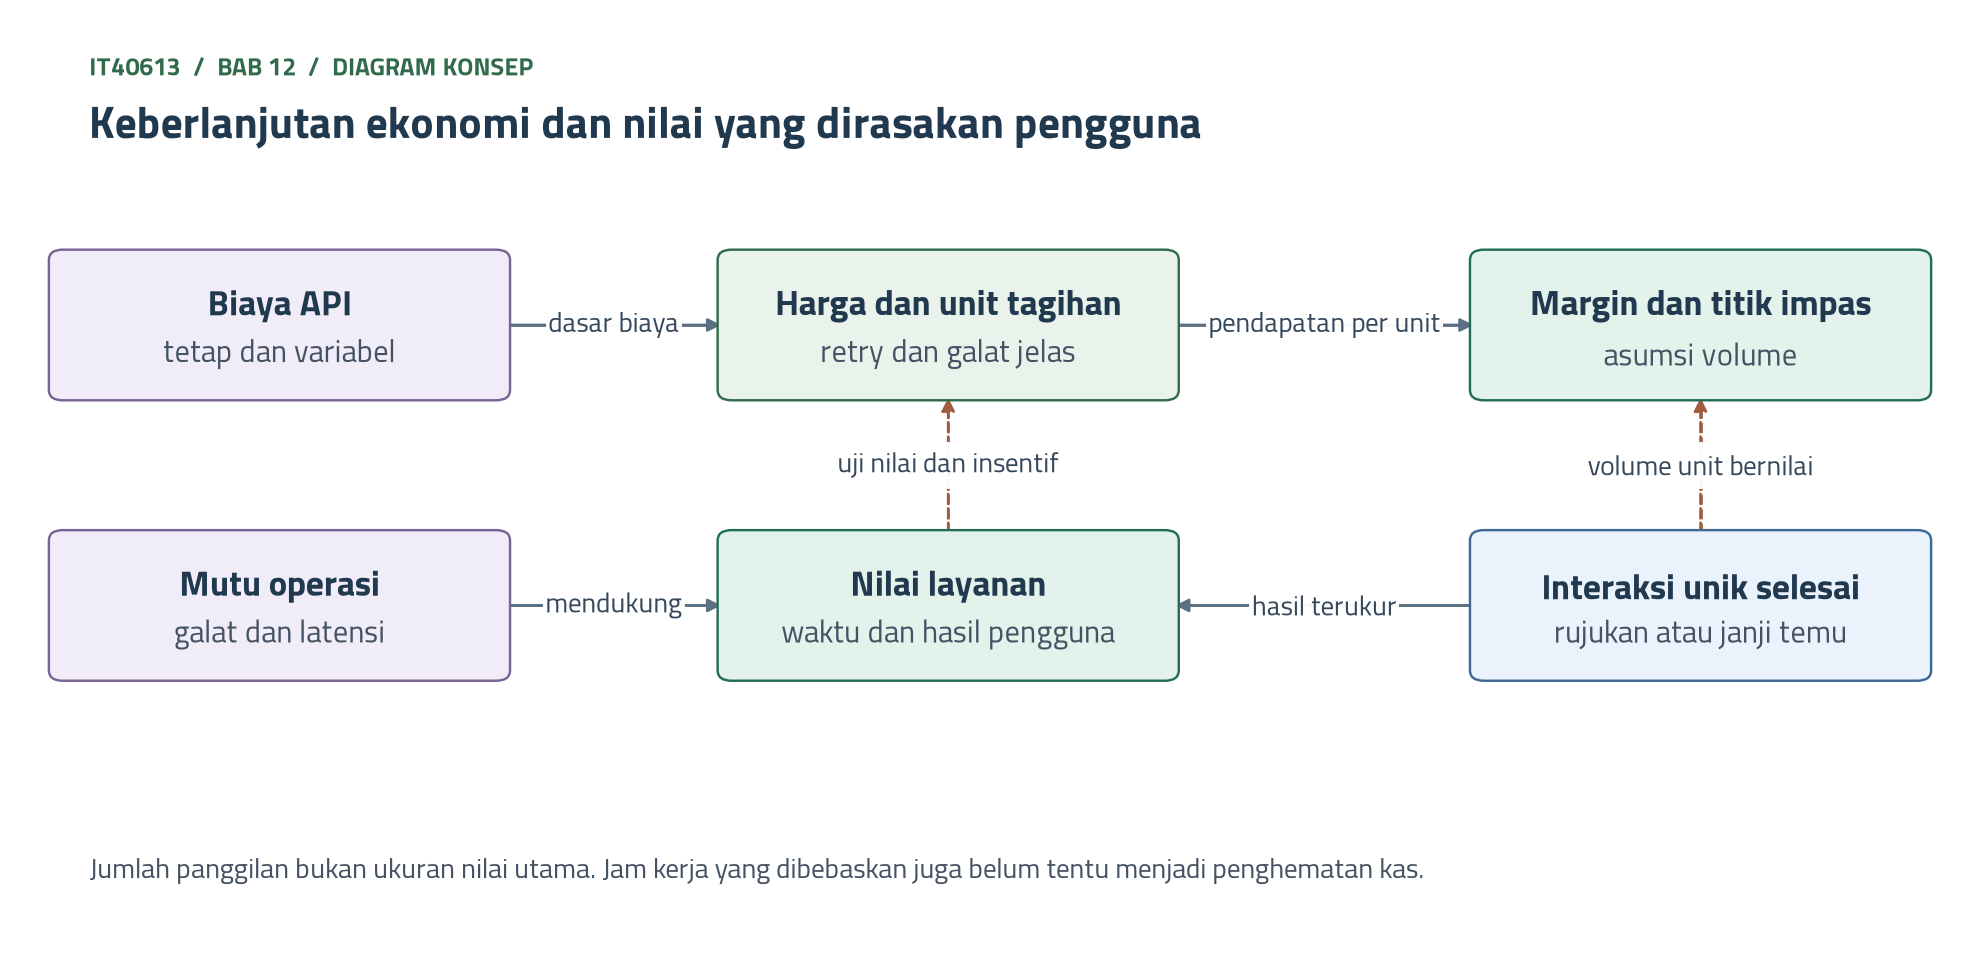
\includegraphics[width=0.96\textwidth,height=0.77\textheight,keepaspectratio]{../../figures/ch12-diagram-konsep.png}
\end{frame}

\begin{frame}{{\Large Masukan dari Bab Sebelumnya}}
  \footnotesize
  \begin{tabularx}{\textwidth}{>{\raggedright\arraybackslash}p{1.3cm} >{\raggedright\arraybackslash}X >{\raggedright\arraybackslash}p{4.4cm}}
    \hline
    \textbf{Asal} & \textbf{Temuan yang dipakai} & \textbf{Kegunaan di sini} \\ \hline
    Bab 2 & Langganan Rp3 juta, verifikasi Rp10.000, biaya Rp2,4 miliar, masa uji 6 bulan & Pembayar dan subsidi \\ \hline
    Bab 4 & API klaim sebagai produk Rp180 juta, setara Rp667 per panggilan & Nilai tidak langsung, unit \\ \hline
    Bab 8 & API-01, telepon 10 ke 2 persen, pemicu 30 klinik & Ukuran dan pemicu \\ \hline
    Bab 10 & Alternatif A rata-rata Rp269,6 juta, Rp60 juta bergantung trafik & Biaya tetap dan variabel \\ \hline
    Bab 11 & P2, SLA 99,0 dan SLO 99,4 persen, U1 sampai U5 & Metrik dan kredit \\ \hline
  \end{tabularx}

  \vspace{8pt}
  \small Tetap dipakai: 40 klinik mitra, kuota 300 per hari per klinik, tarif Rp60.000 per jam, lapisan bersama Rp300 juta per tahun.
\end{frame}

\section{Nilai API}

\begin{frame}{{\Large Nilai Langsung dan Tidak Langsung}}
  \vspace{8pt}
  \begin{itemize}
    \item Nilai langsung: pendapatan yang dapat diatribusikan.
    \item Nilai tidak langsung: saluran, retensi mitra, penghematan proses.
    \item Penghematan waktu tidak otomatis mengurangi kas.
    \item Postman 2025: 65 persen organisasi memperoleh pendapatan dari API. Penerbitnya menjual alat API.
    \item Benzell dkk.: API internal saja tidak menunjukkan efek signifikan pada ukuran pertumbuhan.
  \end{itemize}
  \vspace{6pt}
  {\small Analogi: jalan antardesa bernilai karena truk sayur lebih cepat, walaupun tanpa loket tol.}
\end{frame}

\begin{frame}{{\Large Dua Contoh Berangka}}
  \vspace{8pt}
  \begin{itemize}
    \item Misalkan 400 telepon enam menit hilang: 40 jam kapasitas per bulan.
    \item Setara Rp2,4 juta per bulan, atau Rp28,8 juta per tahun. Belum tentu kas.
    \item Paket 200 karyawan Rp100 juta, Medikara menyimpan Rp10 juta.
    \item Mencatat Rp100 juta sebagai nilai API menggelembungkan angka 10 kali.
    \item API-06: tanpa manfaat langsung, tetapi prasyarat. Manfaatnya dicatat di portofolio.
  \end{itemize}
\end{frame}

\begin{frame}{{\Large Yang Sering Tertukar: Kapasitas dan Kas}}
  \footnotesize
  \begin{tabularx}{\textwidth}{>{\raggedright\arraybackslash}p{2.6cm} >{\raggedright\arraybackslash}X >{\raggedright\arraybackslash}p{3.6cm}}
    \hline
    \textbf{Klaim} & \textbf{Contoh Medikara} & \textbf{Bukti yang diminta} \\ \hline
    Pendapatan baru & Verifikasi Rp960 juta per tahun, kontrak belum ada & Tagihan direkonsiliasi \\ \hline
    Kas keluar berhenti & Rp900 juta menjadi Rp705 juta, bila sambungan lama dimatikan & Kontrak lama berakhir \\ \hline
    Kapasitas dialihkan & Telepon 10 ke 2 persen: Rp172,8 juta dari Rp216 juta & Catatan tugas pengganti \\ \hline
    Risiko berkurang & Akses ke 138 tabel dicabut & Temuan audit ditutup \\ \hline
    Kewajiban dipenuhi & 10 sambungan BPJS Kesehatan dan SATUSEHAT, Rp450 juta & Kiriman berhasil \\ \hline
  \end{tabularx}

  \vspace{8pt}
  \small Telepon yang berkurang dan langganan Rp1,44 miliar tidak boleh dijumlahkan: manfaatnya terhitung dua kali.
\end{frame}

\section{Model Harga API}

\begin{frame}{{\Large Lima Model Harga}}
  \footnotesize
  \begin{tabularx}{\textwidth}{>{\raggedright\arraybackslash}p{2.1cm} >{\raggedright\arraybackslash}X >{\raggedright\arraybackslash}X}
    \hline
    \textbf{Model} & \textbf{Risiko} & \textbf{Pada Medikara} \\ \hline
    Gratis & Biaya berjalan tanpa pemilik anggaran & API internal, sambungan wajib \\ \hline
    \textit{Freemium} & Pemakai gratis tidak pernah membayar & Tingkat 0: jadwal tanpa akun, 1.000 panggilan per hari \\ \hline
    Berjenjang & Kapasitas menganggur, lonjakan di atas batas & Paket kecil, sedang, besar \\ \hline
    Per pemakaian & Tagihan sulit diperkirakan & Verifikasi Rp10.000 \\ \hline
    Bagi hasil & Rekonsiliasi rumit, insentif klinis & Paket perusahaan: 10 persen \\ \hline
  \end{tabularx}

  \vspace{8pt}
  \small Analogi: tagihan air mengikuti meter, langganan kelas senam mengikuti paket kehadiran.
\end{frame}

\begin{frame}{{\Large Harga Terbuka: Pelajari Bentuknya, Bukan Besarnya}}
  \footnotesize
  \begin{tabularx}{\textwidth}{>{\raggedright\arraybackslash}p{2.3cm} >{\raggedright\arraybackslash}X}
    \hline
    \textbf{Penyedia} & \textbf{Rincian yang tertulis} \\ \hline
    Stripe & 2,9 persen ditambah 30 sen dolar per transaksi kartu domestik yang berhasil. Tanpa biaya pendaftaran dan bulanan \\ \hline
    Twilio & 0,0083 dolar per segmen pesan singkat, ditambah biaya operator. 0,001 dolar untuk pesan berstatus gagal \\ \hline
    Google Maps Platform & Gratis 10.000, 5.000, atau 1.000 panggilan per produk per bulan. Paket 100 dolar untuk 50.000 panggilan. Potongan mulai 20 persen di atas 100.000 \\ \hline
  \end{tabularx}

  \vspace{8pt}
  \small Diakses 31 Oktober 2026. Harga dapat berubah. Yang berbeda: siapa menanggung transaksi gagal.
\end{frame}

\begin{frame}{{\Large Mengapa Pelanggan Sering Memilih Paket?}}
  \vspace{8pt}
  \begin{itemize}
    \item Lambrecht dan Skiera: bias menyukai tarif tetap lebih penting dan lebih menetap.
    \item Bias itu tidak menaikkan perpindahan pelanggan secara berarti.
    \item Bias menyukai bayar per pemakaian justru menaikkan perpindahan.
    \item Sundararajan: tarif tetap di samping tarif pemakaian selalu menguntungkan bila penagihan punya biaya transaksi.
    \item Kedua artikel tidak khusus API. Dipakai sebagai petunjuk, bukan angka baku.
  \end{itemize}
\end{frame}

\begin{frame}{{\Large Tiga Model untuk API-01: Total Sama, Beban Berbeda}}
  \footnotesize
  \begin{tabularx}{\textwidth}{>{\raggedright\arraybackslash}p{1.7cm} >{\raggedright\arraybackslash}p{1.0cm} >{\raggedright\arraybackslash}p{1.3cm} >{\raggedright\arraybackslash}X >{\raggedright\arraybackslash}X >{\raggedright\arraybackslash}X}
    \hline
    \textbf{Kelompok} & \textbf{Klinik} & \textbf{Janji} & \textbf{Langganan datar} & \textbf{Per janji sah} & \textbf{Berjenjang} \\ \hline
    Kecil & 10 & 500 & Rp3 juta (Rp6.000) & Rp1 juta (Rp2.000) & Rp1,5 juta (Rp3.000) \\ \hline
    Sedang & 20 & 1.500 & Rp3 juta (Rp2.000) & Rp3 juta (Rp2.000) & Rp3 juta (Rp2.000) \\ \hline
    Besar & 10 & 2.500 & Rp3 juta (Rp1.200) & Rp5 juta (Rp2.000) & Rp4,5 juta (Rp1.800) \\ \hline
    \textbf{Per tahun} & \textbf{40} & & \textbf{Rp1,44 miliar} & \textbf{Rp1,44 miliar} & \textbf{Rp1,44 miliar} \\ \hline
  \end{tabularx}

  \vspace{8pt}
  \small Tagihan per bulan, dengan harga efektif per janji dalam kurung. Sebaran klinik adalah pemisalan latihan. Rata-rata tetap 60 janji per hari.
\end{frame}

\begin{frame}{{\Large Tagihan Klinik pada Tiga Model}}
  \centering
  \eadiagram{../../figures/ch12-tagihan-model.tex}
\end{frame}

\begin{frame}{{\Large Yang Sering Tertukar: Kuota dan Unit Tagihan}}
  \footnotesize
  \begin{tabularx}{\textwidth}{>{\raggedright\arraybackslash}X >{\raggedright\arraybackslash}p{1.5cm} >{\raggedright\arraybackslash}X}
    \hline
    \textbf{Jawaban API-01} & \textbf{Ditagih} & \textbf{Alasan} \\ \hline
    201 pertama, satu kunci idempotensi & Ya & Satu janji sah terbentuk \\ \hline
    Jawaban ulang, kunci yang sama & Tidak & Tidak ada janji baru \\ \hline
    409 konflik slot & Tidak & Janji tidak terbentuk \\ \hline
    401 dan 429 & Tidak & Beban dukungan dan kuota \\ \hline
    503 dan 5xx lain & Tidak & Penyedia tidak dibayar atas kegagalannya \\ \hline
  \end{tabularx}

  \vspace{8pt}
  \small Bila ditagih Rp667 per panggilan dan 10 persen diulang: naik sekitar Rp12 juta per bulan tanpa janji baru. Tagihan per janji perlu rekonsiliasi: Rp28,8 juta per tahun.
\end{frame}

\section{Harga dalam Pasar Multi-Sisi}

\begin{frame}{{\Large Siapa yang Membayar?}}
  \vspace{8pt}
  \begin{itemize}
    \item Pembayar tidak harus pihak yang menghasilkan seluruh trafik.
    \item Rochet dan Tirole: struktur harga, bukan hanya tingkat harga, ikut menentukan hasil.
    \item Armstrong: pengaruh antarkelompok, biaya sekaligus atau per transaksi, satu atau beberapa platform.
    \item Evans dan Schmalensee: kedua sisi harus cukup agar platform berhasil diluncurkan.
    \item Subsidi memerlukan batas waktu dan ukuran keberhasilan.
  \end{itemize}
  \vspace{6pt}
  {\small Analogi: tiket pameran gratis karena peserta pameran membayar tempat.}
\end{frame}

\begin{frame}{{\Large Dua Contoh Berangka}}
  \vspace{8pt}
  \begin{itemize}
    \item Pasien Rp10.000 per pemesanan: 30 persen kembali ke telepon, kurang Rp720 juta.
    \item Klinik dan asuransi membayar: Rp2,4 miliar tanpa menekan pemesanan.
    \item Masa uji enam bulan: Rp18 juta per klinik, Rp720 juta untuk 40 klinik.
    \item Bila 28 klinik bertahan: Rp216 juta tidak kembali, subsidi menjadi Rp25,7 juta per klinik.
    \item \textit{Freemium} tanpa batas waktu dan sebagian kemampuan. Masa uji kemampuan penuh dan terbatas waktu.
  \end{itemize}
\end{frame}

\begin{frame}{{\Large Arus Nilai dan Arus Uang}}
  \centering
  \eadiagram{../../figures/ch12-arus-nilai.tex}
\end{frame}

\begin{frame}{{\Large Uji Nilai bagi Klinik}}
  \footnotesize
  \begin{tabularx}{\textwidth}{>{\raggedright\arraybackslash}X >{\raggedright\arraybackslash}p{1.65cm} >{\raggedright\arraybackslash}p{1.45cm} >{\raggedright\arraybackslash}p{1.55cm} >{\raggedright\arraybackslash}p{1.75cm} >{\raggedright\arraybackslash}p{1.75cm}}
    \hline
    \textbf{Kelompok dan model} & \textbf{Nilai telepon} & \textbf{Tagihan} & \textbf{Sisa ditutup} & \textbf{Kunjungan tambahan} & \textbf{Terhadap janji} \\ \hline
    Kecil, datar & Rp120.000 & Rp3 juta & Rp2,88 juta & 72 & 14,4 persen \\ \hline
    Kecil, berjenjang & Rp120.000 & Rp1,5 juta & Rp1,38 juta & 35 & 7,0 persen \\ \hline
    Sedang, kedua model & Rp360.000 & Rp3 juta & Rp2,64 juta & 66 & 4,4 persen \\ \hline
    Besar, datar & Rp600.000 & Rp3 juta & Rp2,4 juta & 60 & 2,4 persen \\ \hline
    Besar, berjenjang & Rp600.000 & Rp4,5 juta & Rp3,9 juta & 98 & 3,9 persen \\ \hline
  \end{tabularx}

  \vspace{8pt}
  \small Marjin Rp40.000 per kunjungan tambahan adalah pemisalan latihan.
\end{frame}

\begin{frame}{{\Large Kasus Medikara: Mengapa Klinik Mau Membayar Rp3 Juta?}}
  \vspace{6pt}
  \begin{itemize}
    \item Telepon yang berkurang hanya 12 persen dari tagihan klinik sedang.
    \item Pasien tetap Rp0 untuk pemesanan. Vendor tidak ditagih.
    \item Klinik memakai paket berjenjang dengan unit janji sah. Paket sedang tetap Rp3 juta.
    \item Masa uji tetap enam bulan. Bagi hasil atas rujukan ditolak untuk saat ini.
    \item Harganya: 20 klinik kecil, 20 sedang, dan 0 besar menurunkan pendapatan menjadi Rp1,08 miliar.
  \end{itemize}
  \vspace{4pt}
  {\small Bukti pengubah keputusan: sebaran nyata, kunjungan tambahan, dan wawancara kesediaan membayar.}
\end{frame}

\section{Biaya dan Titik Impas}

\begin{frame}{{\Large Titik Impas}}
  \vspace{4pt}
  \[
    \text{Volume impas} = \frac{\text{Biaya tetap}}{\text{Harga per unit} - \text{Biaya variabel per unit}}
  \]
  \begin{itemize}
    \item Biaya tetap Rp20 juta, harga Rp500, variabel Rp100: margin Rp400, impas 50.000 unit.
    \item Harga turun menjadi Rp100: margin nol, tidak ada volume yang menutup biaya.
    \item Biaya keamanan, dukungan, dan pengiriman data ikut dihitung.
  \end{itemize}
  \vspace{4pt}
  {\small Analogi: warung menghitung porsi yang menutup sewa setelah biaya bahan dipenuhi.}
\end{frame}

\begin{frame}{{\Large Biaya Tahunan API-01, Juta Rupiah}}
  \footnotesize
  \begin{tabularx}{\textwidth}{>{\raggedright\arraybackslash}p{5.0cm} >{\raggedright\arraybackslash}p{1.2cm} >{\raggedright\arraybackslash}X}
    \hline
    \textbf{Komponen} & \textbf{Nilai} & \textbf{Asal angka} \\ \hline
    Lapisan bersama, bagian tetap & 225,6 & Pagu Rp300 juta dikurangi trafik dan tiket \\ \hline
    Pemilik produk, dukungan, perubahan & 180 & Misalkan setara API klaim Bab 4 \\ \hline
    \textbf{Jumlah tetap} & \textbf{405,6} & \\ \hline
    Trafik, tiket, rekonsiliasi, kredit SLA & 115,2 & 60 + 14,4 + 28,8 + 12: Rp2,88 juta per klinik \\ \hline
    \textbf{Total pada 40 klinik} & \textbf{520,8} & \\ \hline
  \end{tabularx}

  \vspace{8pt}
  \small Harga rata-rata Rp36 juta per klinik per tahun. Margin Rp33,12 juta. Impas 12,25, dibulatkan menjadi 13 klinik.
\end{frame}

\begin{frame}{{\Large Titik Impas Lapisan API-01}}
  \centering
  \eadiagram{../../figures/ch12-titik-impas.tex}
\end{frame}

\begin{frame}{{\Large Kepekaan: Harga Lebih Menentukan daripada Trafik}}
  \footnotesize
  \begin{tabularx}{\textwidth}{>{\raggedright\arraybackslash}X >{\raggedright\arraybackslash}p{2.6cm} >{\raggedright\arraybackslash}p{2.8cm} >{\raggedright\arraybackslash}p{2.0cm}}
    \hline
    \textbf{Skenario} & \textbf{Biaya tetap} & \textbf{Margin per klinik} & \textbf{Titik impas} \\ \hline
    Dasar: Rp3 juta per bulan & Rp405,6 juta & Rp33,12 juta & 13 klinik \\ \hline
    Harga Rp2 juta per bulan & Rp405,6 juta & Rp21,12 juta & 20 klinik \\ \hline
    Harga Rp1 juta per bulan & Rp405,6 juta & Rp9,12 juta & 45 klinik \\ \hline
    Harga Rp240.000 per bulan & Rp405,6 juta & Rp0 & Tidak ada \\ \hline
    Trafik dua kali lipat & Rp405,6 juta & Rp31,62 juta & 13 klinik \\ \hline
    Tim produk dua kali lipat & Rp585,6 juta & Rp33,12 juta & 18 klinik \\ \hline
  \end{tabularx}
\end{frame}

\begin{frame}{{\Large Tiga Volume, Tiga Hasil}}
  \footnotesize
  \begin{tabularx}{\textwidth}{>{\raggedright\arraybackslash}p{1.2cm} >{\raggedright\arraybackslash}X >{\raggedright\arraybackslash}p{1.6cm} >{\raggedright\arraybackslash}p{2.3cm} >{\raggedright\arraybackslash}p{2.5cm}}
    \hline
    \textbf{Asal} & \textbf{Lingkup angka} & \textbf{Janji per bulan} & \textbf{Pendapatan Rp2.000} & \textbf{Terhadap Rp520,8 juta} \\ \hline
    Bab 8 & Skenario atas: seluruh 60 kunjungan per hari lewat API & 60.000 & Rp1,44 miliar & Rp919,2 juta \\ \hline
    Bab 1 dan 5 & Angka dasar: janji temu pada Medikara+ & 28.000 & Rp672 juta & Rp151,2 juta \\ \hline
    Bab 2 & Skenario harga: 240.000 pemesanan per tahun pada 40 klinik mitra & 20.000 & Rp480 juta & Kurang Rp40,8 juta \\ \hline
  \end{tabularx}

  \vspace{8pt}
  \small Impas per janji sah: 21.700 janji per bulan. Per janji memindahkan risiko volume ke Medikara. Langganan datar memindahkannya ke klinik.
\end{frame}

\begin{frame}{{\Large Kasus Medikara: Dua Titik Impas}}
  \vspace{6pt}
  \begin{itemize}
    \item Lapisan API menutup Rp520,8 juta. Platform menutup Rp2,4 miliar.
    \item Pada 28 klinik: lapisan API margin Rp521,76 juta, platform kurang Rp432 juta.
    \item Pada 30 klinik, pemicu Bab 8: platform kurang Rp360 juta.
    \item Tanpa kontrak verifikasi: kurang Rp960 juta. Masa uji menahan langganan tahun pertama menjadi Rp720 juta.
    \item Laporan memisahkan kedua margin. Tagihan murni per janji ditolak pada tahun pertama.
  \end{itemize}
  \vspace{4pt}
  {\small Rincian kelayakan investasi: \textit{business case} di IT40513.}
\end{frame}

\section{Metrik Platform dan Metrik API}

\begin{frame}{{\Large Dua Keluarga Metrik}}
  \vspace{8pt}
  \begin{itemize}
    \item Metrik platform: likuiditas, tingkat kecocokan, aktivasi mitra, retensi.
    \item Metrik API: adopsi, volume panggilan, tingkat galat, latensi.
    \item Keduanya dihubungkan oleh identitas transaksi yang aman.
    \item Tiap klinik: 180 ke 300 panggilan per hari lewat \textit{polling}, tanpa janji baru.
    \item SRE: galat yang lambat lebih buruk. Pisahkan latensi berhasil dari latensi gagal.
  \end{itemize}
  \vspace{6pt}
  {\small Analogi: kecepatan kasir dibaca bersama jumlah pelanggan yang menerima barang sesuai pesanan.}
\end{frame}

\begin{frame}{{\Large Delapan Metrik pada API-01}}
  \scriptsize
  \begin{tabularx}{\textwidth}{>{\raggedright\arraybackslash}p{2.1cm} >{\raggedright\arraybackslash}X >{\raggedright\arraybackslash}p{1.9cm} >{\raggedright\arraybackslash}X}
    \hline
    \textbf{Metrik} & \textbf{Definisi} & \textbf{Contoh} & \textbf{Menyesatkan bila} \\ \hline
    Likuiditas & Pencarian menemukan slot dalam 7 hari & 85 persen & Jadwal kosong ikut dihitung \\ \hline
    Tingkat kecocokan & Pemesanan memperoleh slot tanpa konflik & 90 persen & Sasaran waktu dilonggarkan \\ \hline
    Aktivasi mitra & Minimal satu 201 produksi dalam 30 hari & 28 dari 40 & Klinik memesan uji di produksi \\ \hline
    Retensi & Aktif 6 bulan lalu, masih aktif sekarang & 26 dari 28 & Masa gratis dihitung bertahan \\ \hline
    Adopsi & Memegang kredensial produksi & 34 dari 40 & Kredensial dibaca sebagai pemakaian \\ \hline
    Volume panggilan & Seluruh permintaan per bulan & 84.000 & \textit{Polling} terbaca sebagai pertumbuhan \\ \hline
    Tingkat galat & 5xx dibagi permintaan pemesanan & 0,6 persen & Pemeliharaan dicampur tanpa aturan \\ \hline
    Latensi & Persentil ke-95, pemesanan berhasil & 1.890 ms & Dibaca sebagai rata-rata \\ \hline
  \end{tabularx}
\end{frame}

\begin{frame}{{\Large Membaca Log Gateway Klinik Uji}}
  \footnotesize
  \begin{tabularx}{\textwidth}{>{\raggedright\arraybackslash}p{1.2cm} >{\raggedright\arraybackslash}p{1.8cm} >{\raggedright\arraybackslash}p{1.6cm} >{\raggedright\arraybackslash}p{2.0cm} >{\raggedright\arraybackslash}X}
    \hline
    \textbf{Klinik} & \textbf{Panggilan} & \textbf{Transaksi unik} & \textbf{Panggilan per transaksi} & \textbf{Yang terlihat} \\ \hline
    U1 & 15 & 5 & 3,00 & Pola normal \\ \hline
    U2 & 13 & 4 & 3,25 & Satu 503, lalu berhasil \\ \hline
    U3 & 19 & 3 & 6,33 & Menanyakan jadwal tiap 5 menit \\ \hline
    U4 & 10 & 2 & 5,00 & Dua 503, satu 409 \\ \hline
    U5 & 5 & 0 & Tidak terhitung & Seluruhnya 401, masalah token \\ \hline
  \end{tabularx}

  \vspace{6pt}
  \small Tagihan untuk 14 janji: Rp41.354 per panggilan, Rp28.000 per janji. Median 259 ms, persentil ke-95 1.890 ms, rata-rata 722 ms. Data sintetis.
\end{frame}

\section{North Star Metric dan Pohon Metrik}

\begin{frame}{{\Large North Star Metric}}
  \vspace{8pt}
  \begin{itemize}
    \item Ukuran ringkas nilai berulang bagi pengguna.
    \item Tiga sifat: mewakili nilai, dalam jangkauan tim, mendahului pendapatan.
    \item Pendorong biasanya tiga sampai lima. Ukuran utama tidak digerakkan langsung.
    \item Medikara: janji temu dan rujukan selesai tepat waktu per bulan. Satu ID janji dihitung sekali.
    \item Dasar: 28 klinik, 1.000 pemesanan, 90 dan 80 persen, hasilnya 20.160. Sasaran 34.884.
  \end{itemize}
  \vspace{6pt}
  {\small Analogi: bedakan hasil panen dari jumlah pupuk yang dibeli. Rumusan dari vendor Amplitude, praktik industri.}
\end{frame}

\begin{frame}{{\Large Pohon Metrik API-01}}
  \centering
  \eadiagram{../../figures/ch12-pohon-metrik.tex}
\end{frame}

\begin{frame}{{\Large Pendorong Mana yang Didahulukan?}}
  \footnotesize
  \begin{tabularx}{\textwidth}{>{\raggedright\arraybackslash}X >{\raggedright\arraybackslash}p{1.6cm} >{\raggedright\arraybackslash}p{1.6cm} >{\raggedright\arraybackslash}p{2.2cm} >{\raggedright\arraybackslash}p{2.7cm}}
    \hline
    \textbf{Pendorong} & \textbf{Dasar} & \textbf{Sasaran} & \textbf{Kenaikan diuji} & \textbf{Hasil naik} \\ \hline
    Klinik aktif & 28 & 36 & 1 klinik & 720 (3,6 persen) \\ \hline
    Pemesanan per klinik & 1.000 & 1.200 & 100 pemesanan & 2.016 (10 persen) \\ \hline
    Tingkat kecocokan & 90 persen & 95 persen & 5 poin & 1.120 (5,6 persen) \\ \hline
    Selesai tepat waktu & 80 persen & 85 persen & 5 poin & 1.260 (6,3 persen) \\ \hline
  \end{tabularx}

  \vspace{8pt}
  \small Satu klinik tambahan terlihat kecil, tetapi membawa Rp36 juta per tahun. Paket Rp3 juta setara Rp4.167 per interaksi pada keadaan dasar, dan Rp3.096 pada sasaran.
\end{frame}

\begin{frame}{{\Large Kasus Medikara: Panggilan Naik, Janji Selesai Turun}}
  \vspace{6pt}
  \begin{itemize}
    \item Panggilan 84.000 ke 126.000. Kunjungan portal 4.000 ke 5.200.
    \item Klinik aktif tetap 28. Kecocokan 90 ke 87,5 persen. Selesai 20.160 ke 19.600.
    \item Penyebab: satu vendor memasang \textit{polling}. Panggilan per pemesanan 3 ke 4,5.
    \item Bila ditagih per panggilan: tambah sekitar Rp28 juta per bulan saat nilai turun.
    \item Keputusan: \textit{cache} dan kuota pembacaan, panel pertama diganti, sasaran tanpa jumlah panggilan.
  \end{itemize}
\end{frame}

\section{Metrik Semu}

\begin{frame}{{\Large Metrik Semu dan Penggantinya}}
  \footnotesize
  \begin{tabularx}{\textwidth}{>{\raggedright\arraybackslash}p{2.9cm} >{\raggedright\arraybackslash}X >{\raggedright\arraybackslash}X}
    \hline
    \textbf{Metrik semu} & \textbf{Naik tanpa nilai karena} & \textbf{Pengganti} \\ \hline
    Jumlah panggilan & \textit{Polling}, pengulangan, penolakan & Interaksi unik selesai \\ \hline
    Klinik terdaftar & Kredensial tidak pernah dicabut & 201 produksi dalam 30 hari \\ \hline
    Kunjungan portal & Petugas tersesat dan mengulang & Tugas selesai tanpa bantuan \\ \hline
    Jumlah \textit{endpoint} & Operasi kecil dipecah & Kemampuan yang dipakai mitra \\ \hline
    Rata-rata latensi & Jawaban gagal yang cepat & Persentil ke-95 jawaban berhasil \\ \hline
  \end{tabularx}

  \vspace{8pt}
  \small Ketika ukuran menjadi sasaran, ukuran itu berhenti menjadi ukuran yang baik. Analogi: kartu anggota perpustakaan bukan buku yang dibaca.
\end{frame}

\begin{frame}{{\Large Empat Pertanyaan Sebelum Masuk Dashboard}}
  \vspace{8pt}
  \begin{enumerate}
    \item Keputusan apa yang berubah bila angka ini turun separuh?
    \item Dapatkah angka ini naik tanpa manfaat bagi pengguna?
    \item Siapa pemiliknya, dan apa tindakannya saat angka memburuk?
    \item Apakah definisinya dikunci, dan perubahannya dicatat dengan tanggal?
  \end{enumerate}
  \vspace{6pt}
  {\small Sasaran waktu 7 ke 14 hari: selesai tepat waktu 80 ke 92 persen, tanpa pasien yang dilayani lebih cepat.}
\end{frame}

\begin{frame}{{\Large Lima Pertanyaan Keputusan}}
  \centering
  \eadiagram{../../figures/ch12-peta-keputusan.tex}
\end{frame}

\section{Aktivitas}

\begin{frame}{{\Large Aktivitas: Model Monetisasi dan Pohon Metrik}}
  \vspace{4pt}
  \begin{itemize}
    \item Tujuan: model monetisasi dan pohon metrik satu API mitra sebagai artefak C4.
    \item Anggota bisnis dan akuntansi: biaya, pendapatan, dan titik impas.
    \item Anggota teknis: sumber data tiap metrik di \textit{gateway} atau portal.
    \item Tim: uji nilai bagi pembayar, satu ukuran utama, pendorong, dan penyeimbang.
    \item Kaitan: tonggak C4 Peta Jalan dan Tata Kelola. Kriteria: 25, 30, 30, dan 15 persen.
  \end{itemize}
  \vspace{4pt}
  {\footnotesize Berkas pendukung: \berkas{sources/chapter12/README.md}. Pakai data sintetis, atau data berizin yang dianonimkan.}
\end{frame}

\section{Ringkasan}

\begin{frame}{{\Large Ringkasan}}
  \vspace{4pt}
  \begin{itemize}
    \item Pisahkan kapasitas dari kas, dan jangan menghitung satu manfaat dua kali.
    \item Unit tagihan menentukan siapa menanggung kegagalan. Total Rp1,44 miliar dapat dibagi berbeda.
    \item Struktur harga ikut menentukan hasil. Pasien Rp0, klinik berjenjang, subsidi punya syarat berhenti.
    \item Lapisan API-01 impas pada 13 klinik, tetapi itu bukan titik impas platform.
    \item Tagih dan ukur hal yang dihargai pengguna: layanan selesai, bukan panggilan yang lewat.
  \end{itemize}
\end{frame}

\section{Latihan}

\begin{frame}{{\Large Latihan}}
  \vspace{8pt}
  \begin{enumerate}
    \item Jelaskan mengapa API internal yang tidak menghasilkan uang tetap bisa bernilai tinggi, dengan satu contoh dari Medikara.
    \item Bandingkan model bayar per pemakaian dan langganan berjenjang untuk API pengecekan kepesertaan asuransi.
    \item Tentukan satu \textit{north star metric} untuk ekosistem mitra Medikara, lalu jelaskan mengapa jumlah panggilan API bukan pilihan yang tepat.
  \end{enumerate}
  \vspace{8pt}
  {\small Setiap latihan punya tabel contoh dan lembar isian pada Bab 12.}
\end{frame}

\end{document}
